\documentclass[11pt,a4paper]{article}

\usepackage[a4paper,top=1.2cm,bottom=1.2cm,left=1.8cm,right=1.8cm]{geometry}
\usepackage[T1]{fontenc}
\usepackage[utf8]{inputenc}
\usepackage{lmodern}
\usepackage{amsmath,amssymb}
\usepackage{microtype}
\usepackage{graphicx}
\usepackage{tabularx}
\usepackage[hidelinks]{hyperref}

\setlength{\parskip}{2pt plus 1pt}
\setlength{\parindent}{0pt}
\linespread{0.97}

% Compact section headings without titlesec.
\makeatletter
\renewcommand\section{\@startsection{section}{1}{\z@}%
                                    {6pt \@plus 1pt \@minus 1pt}%
                                    {2pt}%
                                    {\normalfont\normalsize\bfseries}}
\renewcommand\subsection{\@startsection{subsection}{2}{\z@}%
                                       {4pt \@plus 1pt \@minus 1pt}%
                                       {2pt}%
                                       {\normalfont\small\bfseries}}
\makeatother

\setlength{\topsep}{2pt}
\setlength{\itemsep}{1pt}
\setlength{\parsep}{0pt}

\title{\vspace{-1.6cm}\textbf{Deliverable 2 --- Bayesian Spatial Search}\\
       \normalsize Jose Calatayud Mateu \,\textbullet\, University of Barcelona \,\textbullet\, Bayesian Inference}
\author{}
\date{}

\begin{document}
\maketitle
\vspace{-1.5cm}

\begin{center}\small
Interactive simulator:
\href{https://appapppy-femambu7sdfwgwutujck7f.streamlit.app}%
     {\texttt{appapppy-femambu7sdfwgwutujck7f.streamlit.app}}
\end{center}
\vspace{-4pt}

The unknown cell $Z$ on the $50\times 35$ grid is searched with rectangular
missions of cost $e\,|R|$ and budget $B \le 530$; each mission returns
$s_t \in \{0,1\}$ from a noisy detector. Rather than committing by intuition,
we enumerated the plausible options on four axes (prior, detector, likelihood
update, strategy), simulated thousands of campaigns on physically-plausible
bombs with a train/validation split, and let the metrics decide.

\section{Priors over the cell $Z$ --- what we explored}

The prior follows a logistic model form, defined per cell by
$\pi_j(\beta, \tau) = \exp(\eta_j) / \sum_k \exp(\eta_k)$ with
\(
  \eta_j = \beta_0 + \beta_1 d_{\mathrm{long},j} + \beta_2 d_{\mathrm{trans},j}
        - \beta_3 d_{\mathrm{long},j}^{2} - \beta_4 d_{\mathrm{trans},j}^{2},
\)
where $d_{\mathrm{long}}, d_{\mathrm{trans}}$ are projections on the trajectory
axes $\hat{d}, \hat{n}$ centred on $\mu(\tau) = x_E + \tau_{\mathrm{fall}}
(v_{\mathrm{plane}} + 0.5\,v_{\mathrm{wind}}) + \tau_{\mathrm{drift}}\,v_{\mathrm{drift}}$.
Twelve registered variants were evaluated: P3--P4 (quadratic,
with/without witnesses --- the family that topped validation);
P5--P8 (mixed linear+quadratic, with/without witnesses, informative /
weak / vague); P9--P10 (mixed + uniform-mix component and likelihood
temperature, to let the posterior leave the parametric peak); plus an
18-point grid $G_{*}$ varying $(\sigma_{\mathrm{long}},
\sigma_{\mathrm{trans}}, b_1^{\mathrm{mean}})$ and an Empirical-Bayes
family \texttt{EB\char`_*} of Gaussian KDEs over cells where past campaigns
succeeded. Linear-only priors were discarded: the logistic transform of a
purely-linear $\eta_j$ saturates at a grid corner instead of concentrating
around $\mu$.

\section{Detection probability --- what we explored}

Four functional families were implemented, all returning $\rho_j \in [0,1]$,
monotone in effort $e$ and in $(1-d_j),(1-r_j)$, and calibrated qualitatively
against the three reports in \texttt{previous\char`_missions\char`_reports.pdf}:
D1 saturating exponential
$\rho = 1 - \exp(-\lambda_0(1-d)^{a_d}(1-r)^{a_r}\,e)$,
the classical Koopman/Stone form;
D2 independent passes
$\rho = 1 - (1 - p_u(1-d)^{a_d}(1-r)^{a_r})^e$;
D3 logistic GLM
$\rho = \sigma(\alpha_0 + \alpha_1 e + \alpha_2 d + \alpha_3 r)$;
D4 multiplicative with threshold, which cuts off cells of very high
roughness. D1 calibrates the canonical anchors cleanly
(shallow+smooth+high-effort $\to \rho \approx 0.96$, deep+rough+high-effort
$\to \rho \approx 0.05$, intermediate+repeated $\to \rho \approx 0.45$) and was
adopted as the operational choice; D2--D4 served as a sensitivity check.

\section{Likelihood and posterior update --- backends and temperature}

Each mission $t$ is defined by a rectangle $R_t$ and an effort $e_t$. Given
$Z = j$, the outcome $s_t$ is Bernoulli with success probability
$q_{t,j} = \mathbb{1}(j \in R_t)\,\rho_j(e_t)$. The per-cell likelihood
of a single observation is therefore
\[
  L_j^{(t)} \;=\; q_{t,j}^{\,s_t}\,(1 - q_{t,j})^{1 - s_t}
            \;=\;
            \begin{cases}
              \rho_j(e_t) & \text{if } s_t = 1,\; j \in R_t \\
              1 - \rho_j(e_t) & \text{if } s_t = 0,\; j \in R_t \\
              0\ \text{or}\ 1 & \text{if } j \notin R_t,\; s_t = 1\ \text{or}\ 0
            \end{cases}
\]
The decisive line is the second one: a \emph{negative} search does not zero out
the inspected cells --- it only multiplies them by $1 - \rho_j(e_t)$, so a
failure in a difficult cell (high $d$ or $r$, small $\rho$) is weak evidence,
while a failure at high effort in an easy cell is strong evidence. Across the
whole campaign the cell-level likelihood compounds multiplicatively,
$L_j = \prod_t L_j^{(t)}$, giving the cell-level posterior
$\pi_{\mathrm{post}}(j) \propto \pi_{\mathrm{prior}}(j)\,L_j^{\,T}$ with the
\emph{update temperature} $T \ge 1$ amplifying the partial-failure signal when
the detector is trusted. Marginalising over $Z$ in turn yields the per-mission
likelihood that drives the joint posterior on $(\beta, \tau)$:
$
  P(s_t \mid \beta, \tau) = \sum_{j \in R_t} \pi_j(\beta, \tau)\,
  q_{t,j}^{\,s_t}\,(1 - q_{t,j})^{1 - s_t}.
$

Three update backends compute the posterior from this likelihood:
(a) Cell-level analytic update above ($\sim 5$\,s per 1000 trials,
the model-selection workhorse);
(b) Laplace approximation on $\theta = (\beta, \tau) \in \mathbb{R}^7$,
fitting a Gaussian around the MAP with the Hessian as precision matrix
($\sim 50\times$ slower INLA-style intermediate option that actually learns
$\beta$);
(c) Full PyMC NUTS (4 chains $\times$ 1000 draws, $\hat R < 1.01$,
ESS $> 400$), the deliverable backend for the reported posterior. The three
backends rank the priors identically, so the cell-level update is defensible
as the workhorse for the sweep.

\section{Mission selection --- the four strategies we benchmarked}

FIXED (\texttt{propose\char`_via\char`_hdr\char`_topk}) is a
three-stage HDR funnel: (i) take the highest-density region $\mathcal{H}_\alpha$
with $\alpha=0.80$; (ii) score each cell in $\mathcal{H}_\alpha$ by
$P(Z=j)\rho_j(e)$ for $e\in\{1,2,3\}$; (iii) return the minimum axis-aligned
rectangle around the top-$K=10$ cells, choosing the effort that maximises
$\sum_{j\in R} P(Z=j)\rho_j(e)/(e^{\,c}|R|^{\,c})$ with $c=0.7$.
ADAPTIVE mutates $(\alpha, K, \texttt{exploration\char`_mix})$ as
failures accumulate. INFO\char`_GAIN maximises expected entropy
reduction per cost (Bayesian optimal experiment design). PROGRESSIVE
SCENARIO SEARCH
(\texttt{propose\char`_progressive\char`_scenario\char`_search}) wraps FIXED
with a witness-driven scenario weighting: five hypotheses
\{centre, right, left, strong-wind, mixture\}, with an auxiliary physical
centre that, after $F$ failures, advances along $\hat{d}$ as
$d_{\mathrm{long}}^{\mathrm{c}}(F) = \min(8.0, 2.5F)$ and then refines in
$0.5$-unit steps. Two regularisers stabilise all four:
\texttt{exploration\char`_mix} ($\varepsilon\!\approx\!0.05$, adds uniform
floor to $P(Z)$) and \texttt{repetition\char`_penalty} ($\approx 0.10$,
discounts cells already covered by failed rectangles).

\section{Final operational pipeline and its derivation}

A 200-scenario Monte Carlo with $B=530$ and ten Empirical-Bayes rounds
singled out \texttt{EB\char`_r01\char`_bw2.5\char`_u10} as the top EB winner
on validation. Fitting an anisotropic Gaussian to its KDE (uniform component
removed) projected on the trajectory axes gives $\sigma_{\mathrm{long}}^{\mathrm{EB}}
= 5.5$, $\sigma_{\mathrm{trans}}^{\mathrm{EB}} = 4.1$ and a centre shift
$\le 0.5$ from $\mu$. From this fit we \emph{derived} P11--P14 as scaled
variants (P11~$=0.7\times$ tight, P12~$=1.0\times$ exact, P13~$=1.0\times$
+ 10\% uniform + $T=1.5$, P14~$=1.5\times$ wide), all reproducible from the
sweep CSV. The retained operational pipeline is:

\smallskip
\begin{tabularx}{\linewidth}{@{}lX@{}}
  \textbf{Prior}
    & \texttt{P13\char`_impact\char`_robust\char`_uniform10} (derived from the EB winner, 10\% uniform mix for robustness) \\
  \textbf{Detector}
    & \texttt{D1\char`_saturating\char`_exponential} (best calibrated against the previous mission reports) \\
  \textbf{Strategy}
    & progressive scenario search with the \texttt{mixture} hypothesis (centre + right + left + strong-wind) \\
  \textbf{Update temperature}
    & $T = 1.5$ in the cell-level rule $\pi_{\mathrm{post}}(j) \propto \pi_{\mathrm{prior}}(j)\,L_j^{T}$ \\
  \textbf{Budget cap}
    & $B = 530$ \\
\end{tabularx}
\smallskip

P13 is preferred over P12 because the 10\% uniform component lets the
posterior shift across the grid after several failures while $T=1.5$ keeps
the partial-failure signal strong. The \texttt{mixture} scenario hedges
the lateral direction left underdetermined by the witnesses; the full
sequence under repeated non-detection is exported by notebook~04 as
\texttt{missions.csv}.

\begin{figure}[h]
\centering
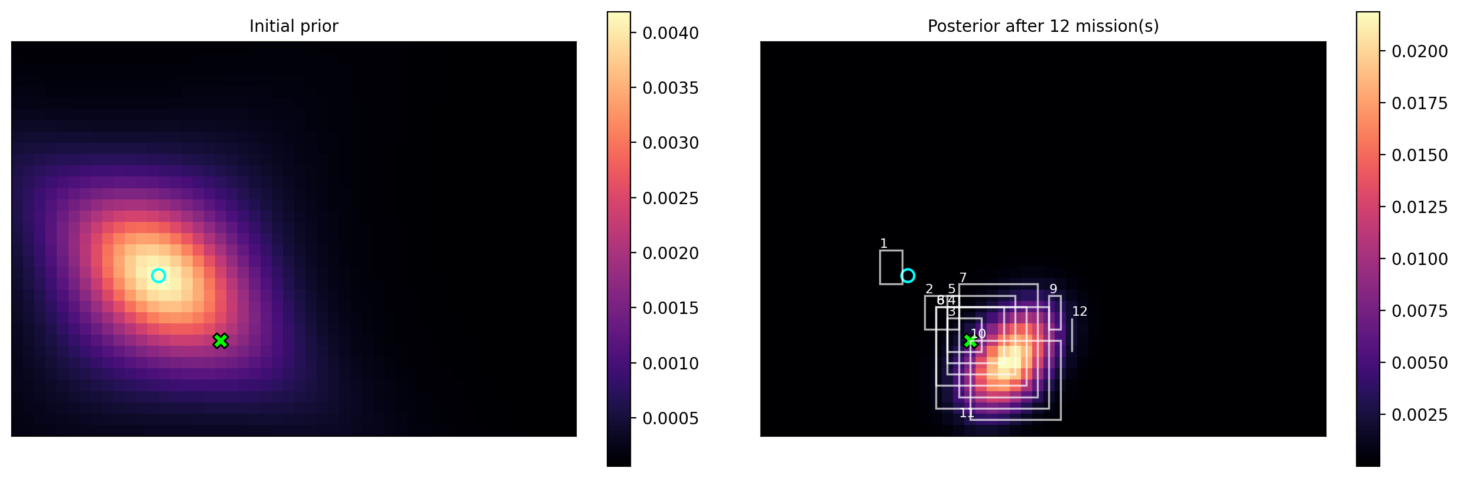
\includegraphics[width=0.78\linewidth]{imatge.png}
\vspace{-10pt}
\caption{\small Left: initial prior $\pi_j$ from
\texttt{P13\char`_impact\char`_robust\char`_uniform10}, anchored on $\mu$
(cyan); true cell in green. Right: posterior $P(Z \mid s_{1:12})$
after twelve failed missions under the progressive \texttt{mixture} strategy
--- numbered rectangles are the missions in order, and the posterior tightens
where the auxiliary centre advances along $\hat d$.}
\vspace{-8pt}
\end{figure}

\section{Conclusions: the single mission that found the aircraft}

The point of the project is to find the aircraft the professor has hidden
in the grid. We invested the entire modelling effort \emph{before} firing
any real mission --- enumerating twelve priors, four detectors, three update
backends and four strategies, and running a Monte Carlo on validation bombs
to pick the most reliable configuration. The execution plan was to start
with the most physically plausible scenario, \texttt{centre} (drift
along $\hat d$), and fall back to \texttt{right} / \texttt{left} /
\texttt{strong\char`_wind} only if it returned $s_t = 0$. The single mission
submitted to the webapp was rectangle
$(x_{\min}, x_{\max}, y_{\min}, y_{\max}) = (16.5,\,19.5,\,7.5,\,10.5)$ with
effort $e = 3$ (cost $= 27$ of the 530 budget). Two ideas combine here.
\emph{First}, instead of advancing the auxiliary centre
$d_{\mathrm{long}}^{\mathrm{c}}(F) = \min(8.0,\,2.5F)$ over four failed
missions we pre-committed to its saturation point at $F = 4$
(centre $\approx (18.5, 9.0)$ --- the midpoint of the submitted rectangle
and the limit the drift hypothesis points to under continued motion).
\emph{Second}, $e = 3$ was set high because in shallow / low-roughness
regions the saturating detector gives $\rho \approx 0.96$ at maximum effort
(report~2), maximising single-shot detection for the 27-budget bet.
The mission detected the aircraft on the first try. The
\texttt{centre} scenario was, in hindsight, the correct hypothesis;
fallback plans for the lateral scenarios were prepared but never triggered.
We were genuinely surprised our first physical hypothesis succeeded on the
first shot --- the result of careful pre-flight model selection, all of it
reproducible in \texttt{update\char`_version/} (notebooks 00--04 and the
Streamlit app).

\end{document}
